\section{Forschungsfragen}

\begin{figure}
    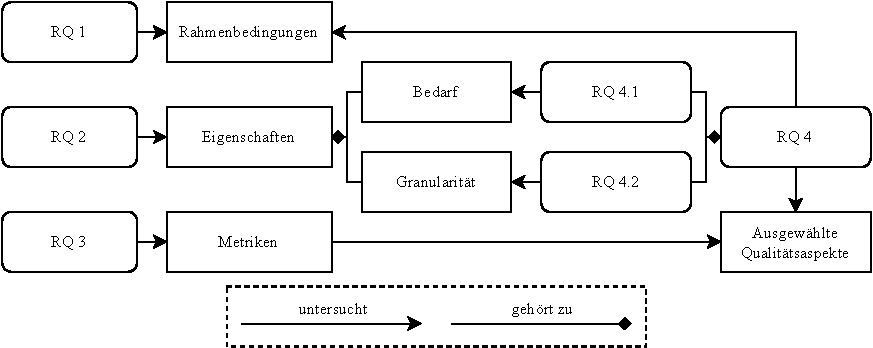
\includegraphics{contents/03_research_design/res/research_questions_overview.pdf}
    \label{fig:research_questions_overview}
    \caption{Abhängigkeiten der Forschungsfragen}
\end{figure}

\noindent\fbox{
    \parbox{\textwidth}{
        \smallskip
        \textbf{RQ1} Welche Randbedingungen haben einen Einfluss auf die Anforderungen für Erklärungen?
        \smallskip
    }
}

\noindent\fbox{
    \parbox{\textwidth}{
        \smallskip
        \textbf{RQ2} Welche Eigenschaften von Erklärungen haben einen Einfluss auf die externe Qualität eines erklärbaren Systems?
        \smallskip
    }
}

\noindent\fbox{
    \parbox{\textwidth}{
        \smallskip
        \textbf{RQ3} Anhand welcher Metriken kann gemessen werden, ob die in ein erklärbares System integrierten Erklärungen das Ziel der Integration erfüllt haben?
        \smallskip
    }
}

\noindent\fbox{
    \parbox{\textwidth}{
        \smallskip
        \textbf{RQ4.1} Welchen Einfluss haben der Kontext und die Zielsetzung eines erklärbaren Systems auf den Bedarf für Erklärungen in Bezug auf die externe Qualität des Systems, wenn Erklärungsbedarf besteht?
        \smallskip
    }
}

\noindent\fbox{
    \parbox{\textwidth}{
        \smallskip
        \textbf{RQ4.2} Welchen Einfluss haben der Kontext und die Zielsetzung eines erklärbaren Systems auf die Granulariät von Erklärungen in Bezug auf die externe Qualität des Systems, wenn Erklärungsbedarf besteht?
        \smallskip
    }
}